%!TEX root = jt-thesis-main.tex

\section{English Abstract}
\begin{onehalfspace}
	
	The english abstract is required for all english theses at TU-Berlin.
\end{onehalfspace}
\clearpage

\section{Deutscher Abstract}
\begin{onehalfspace}
	
	Ein deutscher Abstract wird immer benötigt, für alle Abschlussarbeiten an der TU-Berlin. 
\end{onehalfspace}
\clearpage

\section{Introduction}
\label{sec:Introduction}
% cite: ~\cite{hirzel2014catalog}
% footnote \footnote{footnotes working fine} Author/Rightsholder. (Year). Title of data set (Version number) [Description of form]. Location: Name of producer
Gartner Inc. states that the number of interconnected devices will reach 20.4 billion by 2020 \footnote{Gartner Inc., R. (2017, February 7). Gartner Says 8.4 Billion Connected "Things" Will Be in Use in 2017, Up 31 Percent From 2016. Retrieved September 28, 2018, from https://www.gartner.com/en/newsroom/press-releases/2017-02-07-gartner-says-8-billion-connected-things-will-be-in-use-in-2017-up-31-percent-from-2016}.
To gather information from those devices, we need algorithms which efficiently sample and route data from sensor nodes (i.e., devices) to data sinks. Energy expenditure will gain higher importance, especially for mobile devices such as battery-powered wearables and smartphones. A \ac{WSN} is often battery-powered and use cases span from home and health applications to the military sector~\cite{akyildiz2002wireless}. With low production costs of a node as a goal in \acp{WSN}~\cite{akyildiz2002wireless}, resource usage at the nodes is restricted. While reducing sampling frequencies leads to a higher life of a battery-powered sensor network, important changes in the observed phenomenon could be missed which reduces the quality of the data~\cite{akyildiz2002wireless}. A tradeoff between the quality of data and energy expenditure arises, thus an optimization is needed. Different methods for optimizing \acp{WSN} were presented in surveys (e.g.,~\cite{abbasi2007survey},~\cite{sivrikaya2004time},~\cite{carrano2014survey}). The proposed areas of optimization include clustering algorithms~\cite{abbasi2007survey}, time synchronization~\cite{sivrikaya2004time}, duty cycling~\cite{carrano2014survey}, topology control~\cite{li2013survey}, in-network aggregation~\cite{fasolo2007network}, data compression~\cite{srisooksai2012practical}, and general routing techniques~\cite{al2004routing}~\cite{kulkarni2011particle}~\cite{singh2015survey}~\cite{rault2014energy}. TinyDB~\cite{madden2005tinydb}, ACQUIRE~\cite{sadagopan2003acquire} and COUGAR~\cite{yao2002cougar} introduce system architectures for query processing which consist of algorithms for sampling, and routing data requested by a user through a SQL-like language.




\subsection{Motivation}
\label{sec:motivation}

As stated above, surveys and taxonomies were presented for different areas of sensor networks. However, during our research, we did not encounter a survey or catalog focusing on sampling algorithms in sensor networks. This thesis aims to provide a catalog for a comprehensive overview of the existing sampling algorithms for the specific use case of sensor data. For researchers as well as practitioners, a collection of sampling algorithms is a valuable starting point for finding a solution for a design problem in a sensor network. Thus, a taxonomy of the algorithms will be presented to provide a compact overview. Furthermore, algorithms which focus on areas other than sensing (like routing and topology building) in sensor networks will be presented. Combinations of said algorithms with sampling algorithms as well as combinations of sampling algorithms from different categories could inspire further research.

\subsubsection{Scientific Background}
\label{sec:Scientific Background}

Different types of \acp{SN}, like \acp{WSN}, \acp{RSN}, or wired \acp{SN} exist. While all of them are used to monitor a phenomenon, like the temperature in a room \footnote{Madden, S. et al. 2004. Intel Lab Data. [ONLINE] Available at: http://db.csail.mit.edu/labdata/labdata.html. [Accessed 29 November 2018].} or the behaviour of wildlife~\cite{bennett2011cranetracker} performance indicators vary in their significance. Intuitively, wired \acp{SN} do not consider energy expenditure as the primary concern. \acp{RSN} have a way to collect energy from the environment they are stationed at, through, e.g. solar and wind or more exotic variants like vibration \footnote{Perpetuum. 2018. Technology. [ONLINE] Available at: https://perpetuum.com/technology/. [Accessed 29 November 2018].}. To enable perpetual data collection in \acp{RSN}, techniques for allocating sensing tasks to sensors while handling the non linear emission of, e.g. solar and wind is crucial~\cite{liu2011perpetual}. \acp{WSN} often have a limited energy source at their disposal, making management of energy expenditure a top priority to increase network lifetime. As Cheng et al. state in their work~\cite{cheng2013stcdg} network lifetime is often defined in \acp{WSN} as the lifetime of the first node to run out of energy. 
% Maybe add different application types: e.g. query based sensing, event based, time based etc. See Routing techniques in wireless sensor networks: a survey under data reporting
% Maybe add a technical outline what is inside a sensor node, see same paper Figure 1
\acp{WSN} and \acp{RSN} are often designed with some nodes sensing the phenomenon and one or more sink nodes wich transfer the sensed data to a central base station. Based on the type of topology, e.g. a simple star structure\ref{fig:topologies}, sensed data is forwarded to the sink node directly, i.e. in a one-hop manner. More complex topologies, e.g. tree \ref{fig:topologies} or connected star structures, often require to relay sensed data through intermediary nodes to a sink node in a multi-hop fashion, as direct communication paths between sensing and sink nodes are not always possible~\cite{romer2004design}.
In more complex topologies with a lot of intermediary nodes, finding the optimal routing path from sensor node to the sink is not trivial. 
With increasing number of nodes, the complexity of the computation of the optimal route increases, as nodes have multiple neighbors from which to choose the next transmission step. Solving such a problem locally, i.e. nodes compute the next best step, with additional contraints, e.g. minimizing energy expenditure and meet quality of data thresholds can an unfeasible task. On the other hand, outsourcing this task to the basestation could induce a major communication overhead with additional energy expenditure.
Techniques on topology building and routing path finding will be discussed later in the thesis.

\begin{figure}%
    \centering
    \subfloat[Star Topology]{{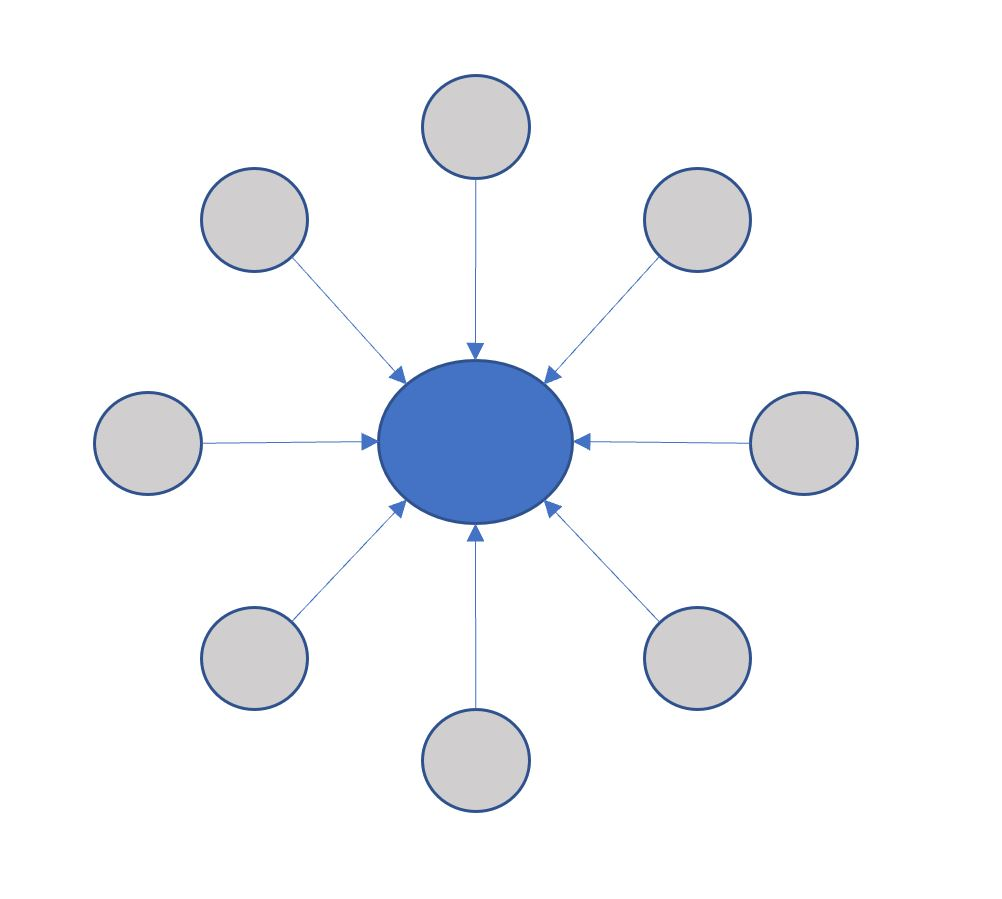
\includegraphics[width=5cm]{images/topology-star-no-legend.jpg} }}%
    \qquad
    \subfloat[Tree Topology]{{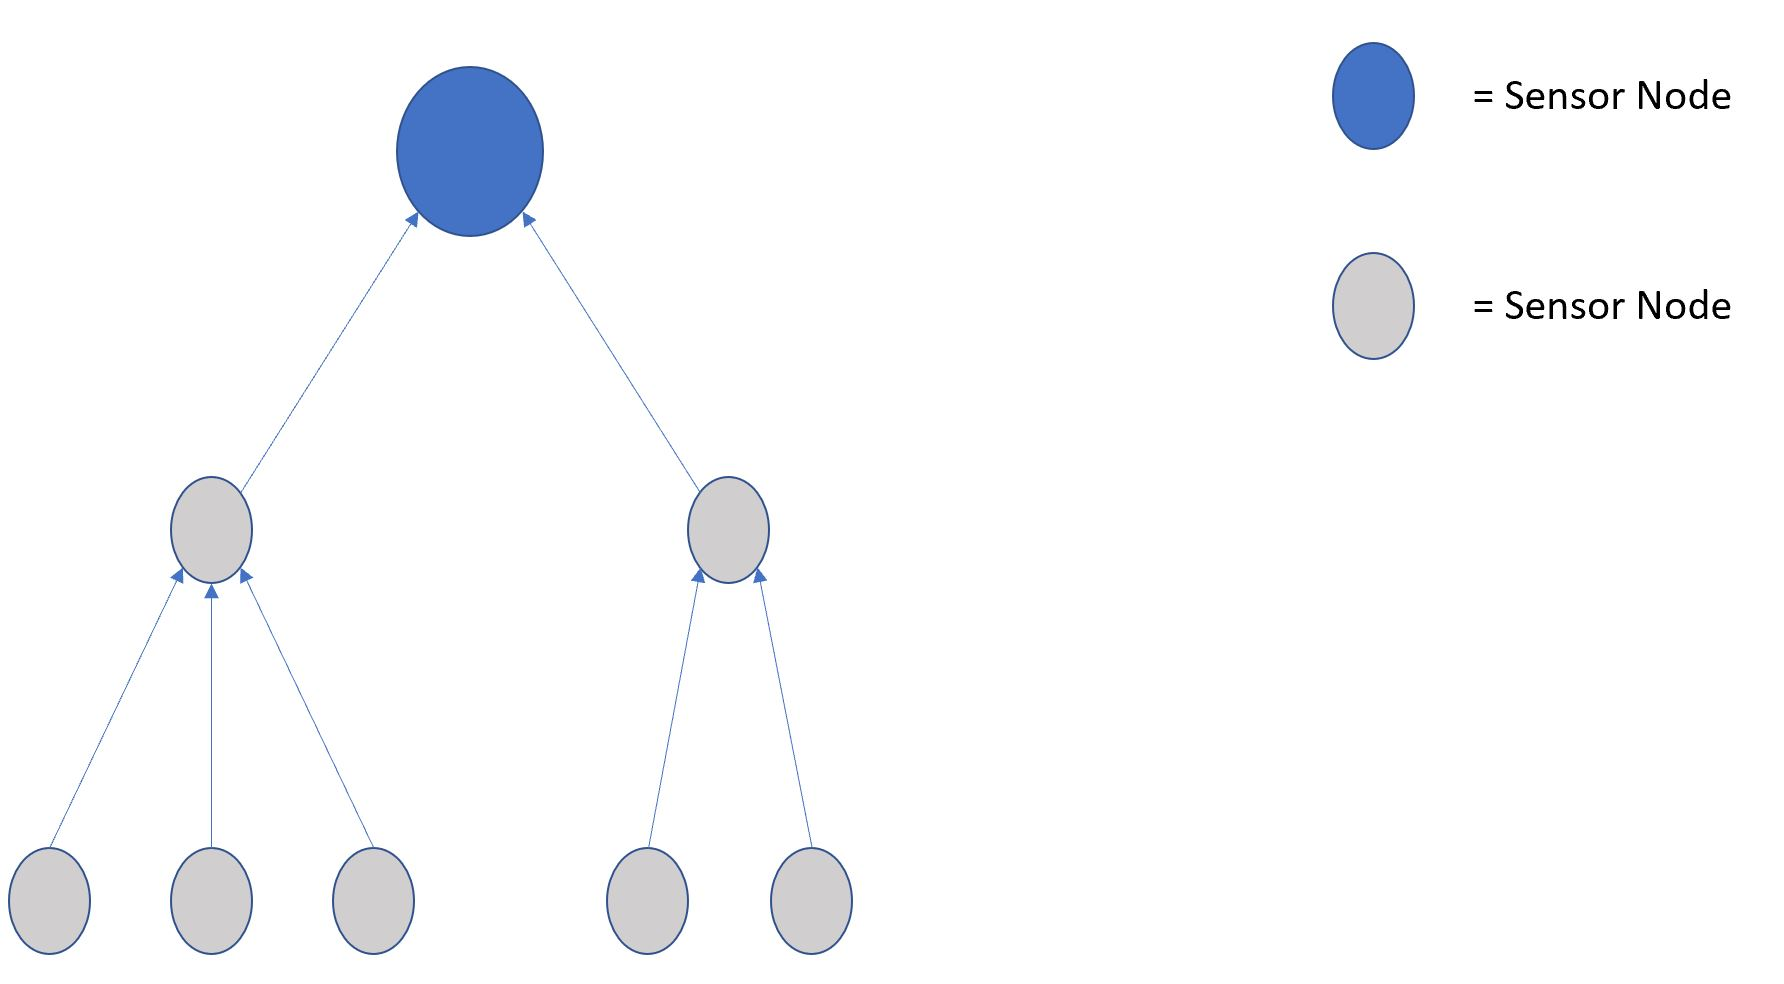
\includegraphics[width=5cm]{images/topology-tree.jpg} }}%
    \caption{Example Topologies. Inspiration taken from Reina et al.~\cite{reina2013role}}%
    \label{fig:topologies}%
\end{figure}

%This command prevents images from being floated too far away.
\FloatBarrier


% However, some algorithms are designed for a specific type of network. For example, AdaM~\cite{trihinas2015adam} can be applied to all kinds of networks, while the algorithm presented by Santini and Romer~\cite{santini2006adaptive} is designed for wireless sensor networks. Other algorithms build upon existing architectures, for example, TiNA~\cite{sharaf2003tina} expands the TinyDB framework with a temporal coherency tolerance to prevent the transmission of slight data changes. Some sampling and filtering algorithms implemented in SNs were initially designed for special use cases and architectures. For example, an algorithm by Alippi et al.~\cite{alippi2010adaptive} was initially designed for a snow monitoring application, however, the authors argue that it is usable in other cases where the monitored phenomenon is slowly changing over time, too. Other algorithms are more general and suited for a range of applications and use cases (e.g.,~\cite{fan2013fast}~\cite{gaura2013edge})


\subsection{Contributions}
\label{sec:contributions}

The contributions of this thesis go as follows: 
\begin{enumerate}
	\item A catalog of different sampling algorithms for sensor data gathering
	\item A taxonomy of those algorithms for a compact overview of the field of data sensing in \acp{SN}
	\item Combinations of different algorithms to provide a basis for further research
\end{enumerate}
\clearpage

\subsection{Thesis Outline}

\para{Section \ref{sec:Background}.}  In section  \ref{sec:Background}, we present ..., including. Furthermore, we provide ... The section concludes with ...

\para{Section X.} Section X provides a survey through related publications. The section is split in two subsections. First, we provide an overview of ... Thereby, we describe ... We conclude with ...

\section{Taxonomy}
\label{sec:Taxonomy}

In this chapter, we present the backgrounds of this thesis. In ... we present ... Add some short introduction to each section.

\subsection{Overview}
\label{sec:Overview}

This is how you can include a figure and refer to it. It is figure \ref{fig:Example}.

\begin{figure}[h!]
	\begin{center}
		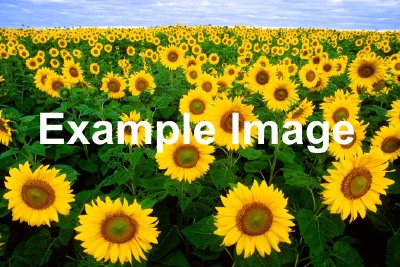
\includegraphics[width=0.5\textwidth]{images/Example.jpg}
		\caption{This is just an example image.}
		\label{fig:Example}
	\end{center}
\end{figure}

%This command prevents images from being floated too far away.
\FloatBarrier

\subsubsection{Adaptive Sampling}
\label{sec:Adaptive Sampling}

This is an example table taken from DIMA's IDB lecture slides:

\begin{table}[h!]
  \begin{tabular}{lccccccc}
	\toprule    
    \hline
    \textbf{Functions} & \multicolumn{3}{c}{\textbf{Framework}} && \multicolumn{2}{c}{\textbf{User Defined}}\\
    \cmidrule{2-4}  \cmidrule{6-7}  
    & Map & Shuffle & Reduce && Mapper &  Reducer\\
    \midrule
    \textbf{Input} & $ (K_m \times V_m)^{*} $ & $ (K_r \times V_r)^{*} $ & $ (K_r \times V_r^{*})^{*} $ && $ (K_m \times V_m) $  & $ (K_r \times V_r^{*}) $\\
    \hline
    \textbf{Output} & $ (K_r \times V_r)^{*} $ & $ (K_r \times V_r^{*})^{*} $ & $ (K_o \times V_o)^{*} $ && $ (K_r \times V_r)^{*} $ & $ (K_o \times V_o)^{*} $\\
	\hline    
    \bottomrule
  \end{tabular}
  \caption{Inputs and outputs of functions and processing phases in Map Reduce.}
  \label{table:mapRedFunctions}
\end{table}

And one more table:

\begin{table}[h!]
  \centering
  \begin{tabular}{lll}
	\toprule    
    \hline
    & \textbf{Input} & \textbf{Output}\\
    \midrule
    File Line 1:& Beer Beer Tea Coffee &\\
    File Line 2:& Tea Tea Beer Tea &\\
	\hline
	Map 1: & (1, Beer Beer Tea Coffee) & [(Beer,1),(Beer,1),(Tea,1),(Coffee,1)]\\
    Map 2: & (2, Tea Tea Beer Tea)     & [(Tea,1),(Tea,1),(Beer,1),(Tea,1)]\\
    \hline
    Reduce 1 & (Beer,[1,1,1])  & (Beer,3)\\  
	Reduce 2 & (Coffee,[1])    & (Coffee,1)\\
	Reduce 3 & (Tea,[1,1,1,1]) & (Tea,4)\\
    \hline    
    \bottomrule
  \end{tabular}
  \caption{Word Count Example: Sample data transformation.}
  \label{table:wcDataTransformation}
\end{table}

\subsubsection{Compressive Sampling}

You may want to use the description environment for your definitions.

Vocabulary introduced by Hirzel et al.~\cite{hirzel2014catalog} and inspired by Gamma et al.~\cite{gamma1995} and Fowler et al.~\cite{fowler1999}.

\begin{description}
	\item[Data Stream] \textit{A conceptual/possibly infinite sequence of data-items which comes from a stream source. Streaming systems implement streams as \ac{FIFO} queues.}
	\item[Stream Source] \textit{A stream source is a data source that possibly emits an infinite number of data-items.}
	\item[Operator] \textit{A code block , which consumes data-items from incoming stream(s) and produces data-items on outgoing stream(s). Thereby it performs a continuous data transformation.}
	\item[Query] \textit{A streaming query consists of operators which are vertices in a graph. The edges of the graph represent the data flow between operators. A streaming query combines multiple operations to a data transformation flow. Queries are also called \textit{applications}.}
	\item[Data-item] \textit{The smallest unit of data, which is processed by the streaming query, is called \emph{data-item}. It is also the smallest unit of communication along edges in the query. Anyhow, data-items can consist of several attributes.}
	\item[Window] \textit{A finite subsequence or chunk of data-items from a stream.}
\end{description}

\subsubsection{Data Sharing}
\label{sec:Listings}

Listing \ref{lst:SPLexample} is an example for a listing using lstlisting.

\begin{lstlisting}[float=b,label=lst:SPLexample,caption={An IBM SPL code example}]
stream<MyType> outputName = Aggregate(InputStream){
	window InputStream : sliding, delta(...), count(...);
	output outputName  : attribute1=Sum(a1*a2), attribute2=Sum(a3);
}
\end{lstlisting}

% Listings can also be imported from files like listing \ref{lst:samplecode}.
% \lstinputlisting[label=lst:samplecode,caption=A Java Hello World Program,language=java]{listings/helloWorld.java}
%Also use: firstline=300,lastline=500, linerange={10-17,20-35}


\section{Discussion}
\label{sec:Discussion}

Lorem ipsum dolor sit amet, consectetur adipisici elit, sed eiusmod tempor incidunt ut labore et dolore magna aliqua. Ut enim ad minim veniam, quis nostrud exercitation ullamco laboris nisi ut aliquid ex ea commodi consequat. Quis aute iure reprehenderit in voluptate velit esse cillum dolore eu fugiat nulla pariatur. Excepteur sint obcaecat cupiditat non proident, sunt in culpa qui officia deserunt mollit anim id est laborum.

\subsubsection{Other Algorithms}
\label{sec:Listings}

Lorem ipsum dolor sit amet, consectetur adipisici elit, sed eiusmod tempor incidunt ut labore et dolore magna aliqua. Ut enim ad minim veniam, quis nostrud exercitation ullamco laboris nisi ut aliquid ex ea commodi consequat. Quis aute iure reprehenderit in voluptate velit esse cillum dolore eu fugiat nulla pariatur. Excepteur sint obcaecat cupiditat non proident, sunt in culpa qui officia deserunt mollit anim id est laborum.


\subsubsection{Combination of Algorithms}
\label{sec:Listings}

Lorem ipsum dolor sit amet, consectetur adipisici elit, sed eiusmod tempor incidunt ut labore et dolore magna aliqua. Ut enim ad minim veniam, quis nostrud exercitation ullamco laboris nisi ut aliquid ex ea commodi consequat. Quis aute iure reprehenderit in voluptate velit esse cillum dolore eu fugiat nulla pariatur. Excepteur sint obcaecat cupiditat non proident, sunt in culpa qui officia deserunt mollit anim id est laborum.


\subsection{Acronyms}
\label{sec:Acronyms}

There are many acronyms provided in this template. You can use them as follows:
\begin{itemize}
	\item \acs{CSV} - The acs-command always uses the short form.
	\item \ac{CSV} - The ac-command uses the long form for the first appearance, then the short form.
	\item \acl{CSV} - The acl-command forces to use the long form.
	\item \acp{CSV} - When adding a 'p' to the mentioned commands, the plural form will be used.
\end{itemize}

\subsection{Citations}
You should read the publications from Albert Einstein~\cite{einstein1920relativity}.

\section{Conclusion}
\label{sec:Conclusion}

It is very important to have a good conclusion.